%==============================================================================
% 五、数据预处理与探索性分析
%==============================================================================
\section{数据核验与预处理}

\subsection{附件的实测结构与题面差异}

八个附件逐行读取后，规模与题面描述并不完全一致。凡有出入处，本文以实测为准，并把差异与处理方式写在下面，避免后续建模建立在错误的量纲与标签之上。

附件1 是化学特征矩阵，$250\times234$，即 250 款酒、3 个元数据列加 231 个化学列。231 列里 5 个是由其他列算出的派生量，含热量值、总酸、总酯、酒花香气与硫化合物。这 5 列保留入模：附件2 的相关矩阵按 231 列给出，剔除派生量会使矩阵与特征表对不上，且派生量本身携带总量信息。231 列的尺度并不统一：37 列经与附件8 的 Calibrated 表逐列对照确认在 $\log_{10}$ 域，33 列确认是原始线性浓度，其余 161 列没有对照、只能按取值范围推定。此外 142 列的含量出现同一检出限地板值，9 列存在真实缺失。

附件2 是化合物相关矩阵，$231\times231$。题面称其为皮尔逊相关，实测是 Spearman：与附件1 重算的 Spearman 矩阵逐格比对，42642 个格子的中位绝对差为 $8.33\times10^{-17}$，与皮尔逊则相差 0.063。因此全文的相关性一律按 Spearman 处理。

附件3 是感官评分卡，题面说 10 个 sheet，实测 13 个。13 张表共 1260 条公式，缓存值全为 0，不提供真值，只提供评分卡结构，含 15 项 Aroma、15 项 Flavour 与 20 个打分项，本文只用其结构。

附件4 是感官标签，$250\times53$，即 3 个元数据加 50 个感官项。它是中心化后的连续强度值，不是 0--6 的整数分，这一点在第六章详述。

附件5 是感官之间的相关矩阵，$50\times50$，同样是 Spearman，行列名用论文长名。

附件6 是化合物与感官的交叉相关矩阵，题面说 $46\times50$，实测 $44\times50$。它只覆盖 $231\times50$ 个可能格子的 18.67\%，因此只作交叉校验，不能当作全量相关结构。

附件7 是论坛评论描述符，$250\times189$，3 列整列为空、可用 183 列，是真正的 $z$ 分数，列标准差中位 1.003。它与附件4 不同源，只用于外部效度检验。

附件8 是综合参考数据，7 个 sheet。其中阈值表 261 行里只有 43 行有数值，这是后文一半归因记录无法做化学判断的直接原因；化学来源标注覆盖 226 个实测特征、余下 5 个派生量归入其他族，用于问题二的分组；Calibrated 表是把 $\log_{10}$ 还原成浓度的官方对照，用于核定量纲；MDI 与 SHAP 两张表是现成的重要性排序，本文不采用，理由见第七章。

最后是题面把"226 种啤酒"写成样本数这一处。全部附件都是 250 行，226 实为化学指标数，本文一律以 250 为样本量。

\subsection{缺失与检出限的分离}

附件1 的缺失有两种不同机制，必须分开处理，这是全文建模的前提。

第一类是检出限截断。有 6807 个单元格的取值精确等于 $-1.817819$，即 $10^{-1.8178}\approx0.0152$，分布在 142 列上。其中 40 列有 30\% 以上的样本精确落在该列的最小值上；若只取最小值恰为检出限 $-1.817819$ 的那 142 列，仍有 35 列的地板值占比超过 30\%。最高的两列（甲基庚烯酮与柠檬烯）达 84.8\%。这表示该化合物低于检测限，是有效信息而非错误值，因此既不删除也不按均值填补。

第二类是真实缺失。按 231 个化学列统计，共 73 个单元格、9 列；去掉 5 个派生列后剩 60 个单元格、8 列，13 格差额全部来自 aroma\_hops\_sum 这一列。缺失最多的 amyl.acetate 占 27/250，且并非随机分布：Dubbel 组 4/10、Kriek 组 3/10、Blond 组 6/31。因此按列中位数填补，不用全表均值，避免把风格差异抹平。这类缺失规模小，不构成建模障碍。

第三类是感官侧的列内左尾。附件4 的标签不是原始 0--6 分值：文献\cite{schreurs2024}的方法写明，16 位品评员先按 7 点量表打分，再\textbf{按品评员做 z-score}（减均值、除标准差），最后按啤酒求平均；原文对此的表述是"Scores were scaled by standard deviation and mean-centered per taster. Values are represented as z-scores"。因此负值表示"低于该品评员的平均"，不是"没有尝到"；列最小值是 z 空间里的左尾，不是感官 0 分。

据此，本文把 $\phi_s$ 定义为\emph{左尾占比}，即与该列最小值相距不超过 0.15 的样本占比
\begin{equation}
  \phi_s=\frac{1}{n}\sum_{i=1}^{n}\mathbb{I}\left(y_{is}\le \min_{i'}y_{i's}+0.15\right),
\end{equation}
作为各列分布左尾厚度的度量，供问题一判断是否需要单独处理高左尾项。图~\ref{fig:q0missing} 给出这两类问题的分栏对比：前者稀疏且集中在少数列，后者是整列高比例的同一取值。

\begin{figure}[htbp]
\centering
\begin{subfigure}[t]{0.48\textwidth}
\centering
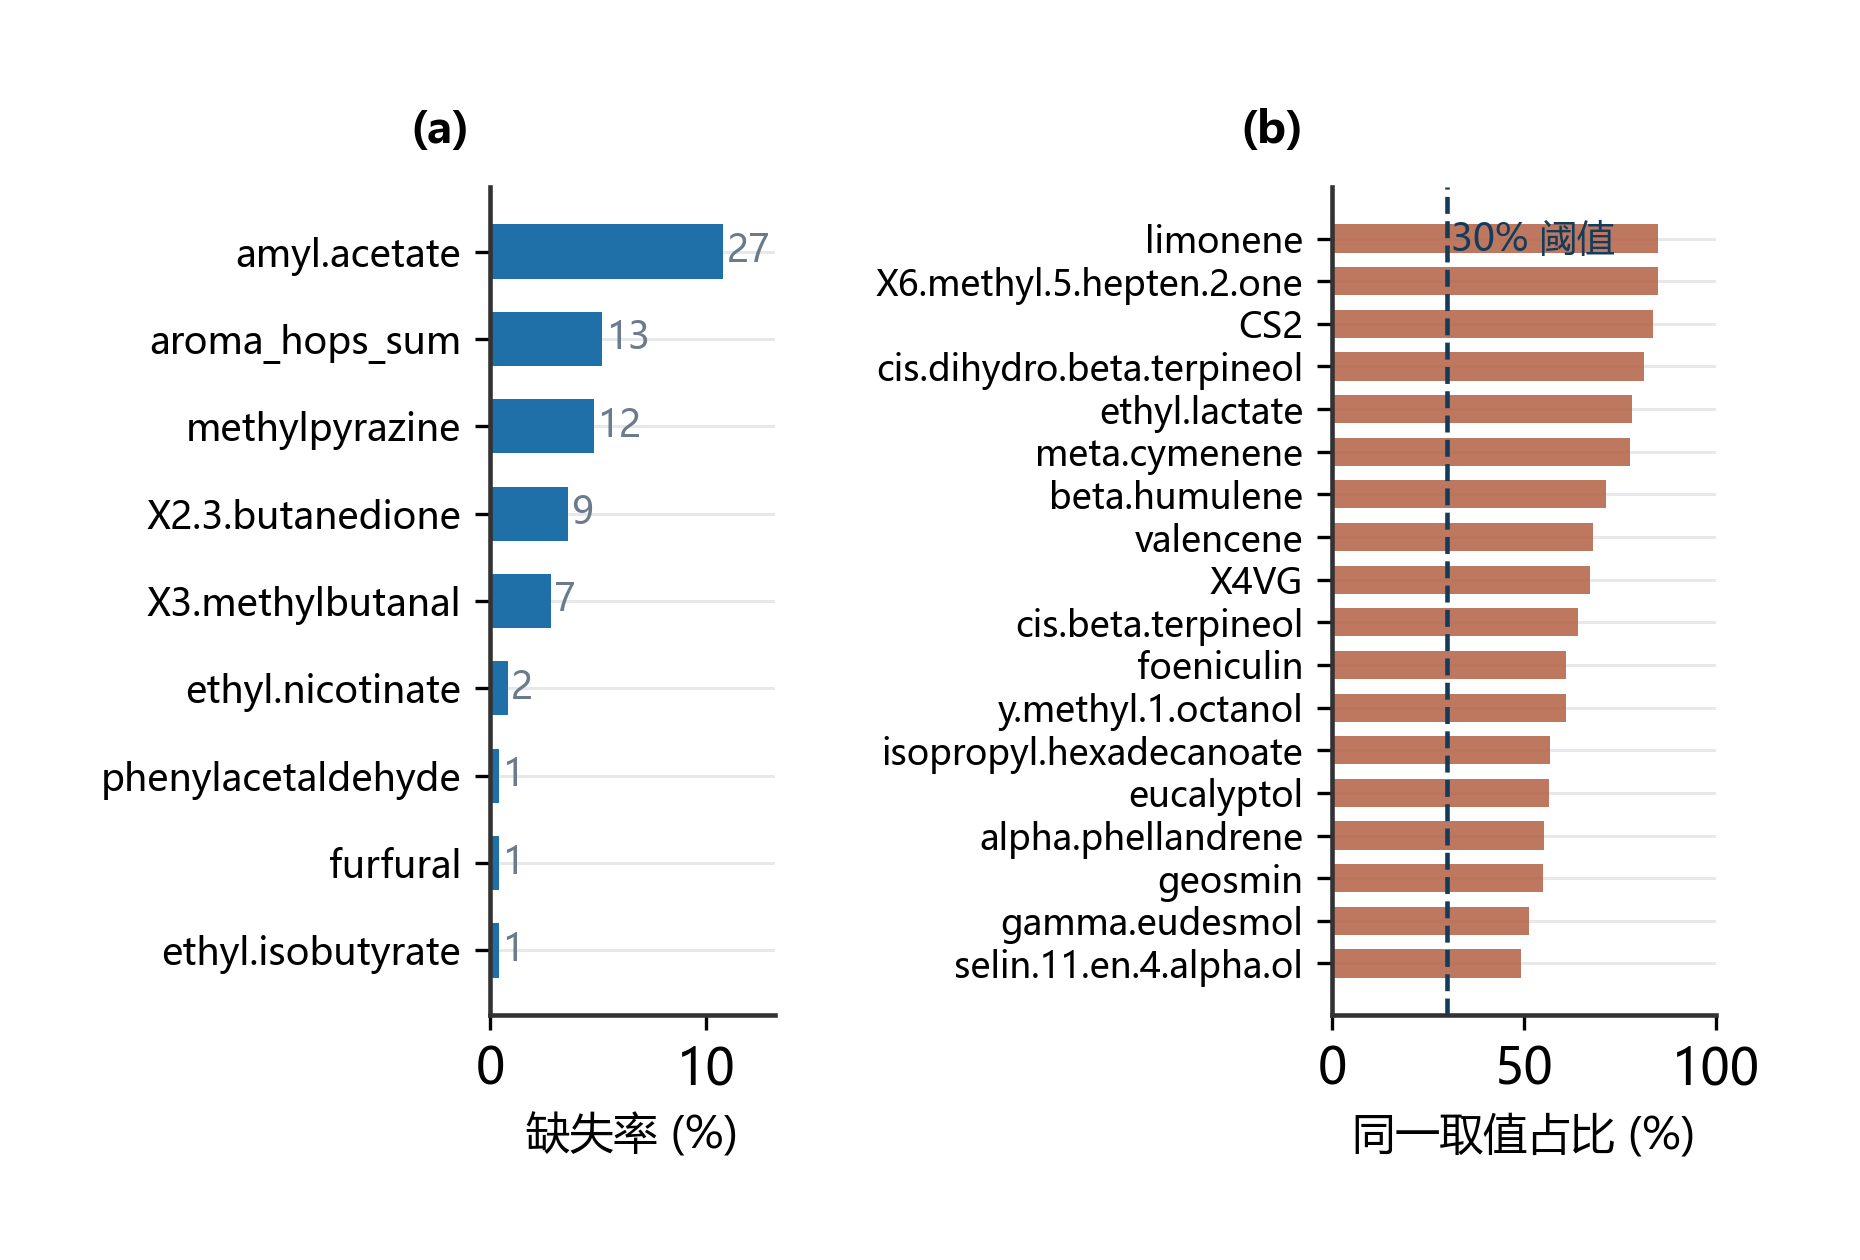
\includegraphics[width=\linewidth]{figures/fig_q0_missing.png}
\caption{数据缺陷的分栏对比。左图为真实缺失列及其缺失率，右图为检出限地板值列，同一取值占比超过 30\% 的列按虚线标出}
\label{fig:q0missing}
\end{subfigure}
\hfill
\begin{subfigure}[t]{0.48\textwidth}
\centering
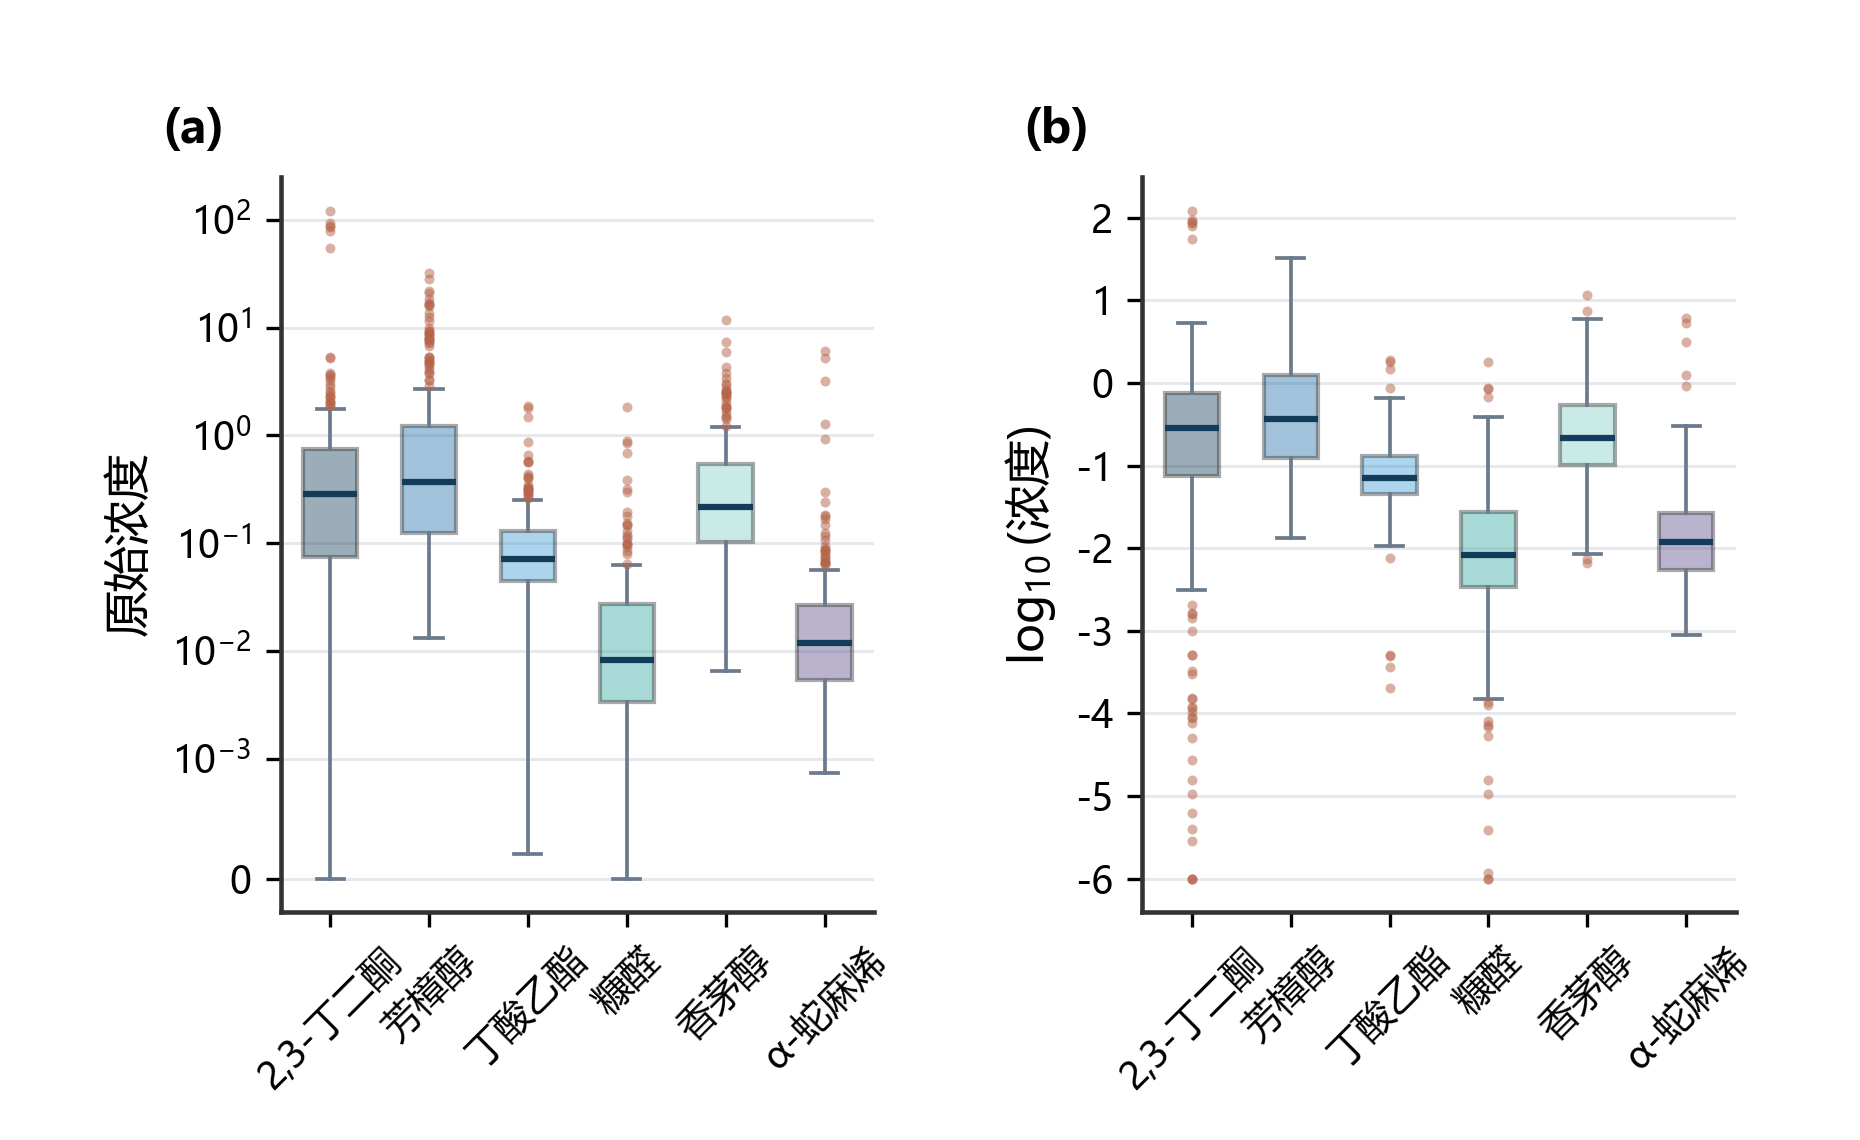
\includegraphics[width=\linewidth]{figures/fig_q0_box_before_after.png}
\caption{量纲统一前后的分布对比。左图为原始浓度对称对数轴，右图为 $\log_{10}$ 域}
\label{fig:q0box}
\end{subfigure}
\caption{数据层面的两处缺陷与处置。左图为真实缺失列的缺失率，右图为量纲统一前后的分布对比（左半为原始浓度对称对数轴，右半为 $\log_{10}$ 域）}
\end{figure}

\subsection{量纲与共线结构}

231 个特征的尺度并不统一，实测分三类：33 列经与附件8 的 Calibrated 表逐列对照，确认是原始线性浓度，相对误差低于 $10^{-3}$ 且列内无零值格；37 列确认在 $\log_{10}$ 域；其余 161 列在 Calibrated 表中没有对照，只能按取值范围判断——145 列含负值，负值只能来自对数域，另 15 列因原始浓度全部大于 1 而取正值、1 列全非负且最小值小于 1 而判为线性域。合计 182 列在 $\log_{10}$ 域、49 列为线性尺度。这个分域不是文字细节：决策变量同时含两种域时，任何“浓度改变量”的求和都必须先归一，具体做法见第八章对 $f_3$ 的说明。

这一点直接决定建模时的处理方式。本文不对任何列做 $10^{x}$ 反变换：反变换后 6 个代表化合物的浓度跨度从 $5.9\times10^{-8}$ 到 121.7，跨越 9 个数量级，标准化虽能把各列压到零均值单位方差，但极端列仍会主导线性模型的系数；保持 $\log_{10}$ 域可把有效跨度压到 6 个数量级左右。图~\ref{fig:q0box} 的左栏即反变换后的原始浓度分布，必须用对称对数轴才能显示，右栏为本文实际使用的 $\log_{10}$ 域分布。



共线的实测结果是本文两处建模选择的直接依据。231 列的方差膨胀因子中位数 35.96、最大 964.91，219 列超过常用阈值 10，其中 31 列超过 100；Spearman 版本的有效秩仅 20.62，条件数 $2.04\times10^5$，需 67 个主成分才达到 90\% 方差，第一主成分只解释 14.48\%。但与此同时，只有 6 对特征的相关系数绝对值超过 0.9，特征对的中位绝对相关仅 0.1293。两者合起来说明：这里的共线是一大片弱相关的累积，不是少数几对强冗余。因此“按方差膨胀因子删变量”会把 219 列删光，正确做法是在建模层面处理——问题二按逐列置换估计重要性，问题三用收缩协方差与偏最小二乘。

\subsection{相关结构与风格差异}

特征与感官之间的关联本身很稀。11550 个特征--感官格子中，中位绝对相关仅 0.0878，超过 0.5 的只有 44 格（0.38\%），超过 0.7 的仅 3 格。表~\ref{tab:senscorr} 列出最强的 5 对，全部可以作化学解释：乙醇对应酒精感与酒体，苦度对应苦味，色度对应焦香麦芽香，辛酸乙酯对应二氧化碳感。

\begin{table}[htbp]
\centering
\footnotesize
\caption{特征与感官的最强相关对，按 Spearman 相关排序}
\label{tab:senscorr}
\begin{tabular*}{\textwidth}{@{\extracolsep{\fill}}llc}
\toprule
\textbf{感官项} & \textbf{化学特征} & $\rho$ \\
\midrule
alcohol & ethanol (v/v) & 0.8171 \\
body & ethanol (v/v) & 0.7191 \\
bitternes & bitterness & 0.6822 \\
A\_malt\_cara & color EBC & 0.5636 \\
co2 & ethyl\_octanoate & 0.5527 \\
\bottomrule
\end{tabular*}
\end{table}

风格的区分力则很强。对 22 个风格做 Kruskal--Wallis 检验，231 个特征中 205 个在 0.05 水平显著、148 个经 Bonferroni 校正后仍显著，效应量 $\varepsilon^2$ 中位 0.1768、最大 0.7910。这既说明风格标签可以作为条件变量使用，这也是问题三可行的依据，也说明若交叉验证不按风格分层，某些折内将不含小类样本，指标会失去意义。

与官方文件的交叉校验达到机器精度：附件2 的 44732 个可比对格子中位绝对差 $8.33\times10^{-17}$，附件6 的 2156 个格子为 $5.55\times10^{-17}$，一致性均为 1。这说明本文的相关矩阵重新计算结果无误，前述共线结构不是实现错误造成的假象。
